\chapter{Motivation}

Traditionally, microcontrollers are programmed in compiled languages such as C or C++. These languages offer high performance and low-level access to hardware, which is important in many embedded applications. However, they can also be difficult to learn and use, especially for beginners.

At Robotárna, branch of a leisure center Helceletka in Brno, we teach programming of microcontrollers to teenagers. To make the learning process easier, we have decided to use a high-level interpreted language -- JavaScript -- instead. While this approach is unconventional, it has a strong advantage of a very fast code-build-test cycle. The speed of this cycle makes it easier for students to maintain their focus and allows them to experiment more with their code.

Because programming in JavaScript as a dynamically typed language can sometimes lead to errors that are difficult to debug, we usually do not write JavaScript directly. Instead, TypeScript is used and compiled to JavaScript before execution.

So far, we have observed success with this approach. We see students being able to learn basics faster and start working on more interesting projects sooner. However, with students creating more complex projects, we have also reached a point where we need to consider performance of JavaScript programs.

JavaScript, as an interpreted language, suffers from the inherent flaw of slow execution speed. It comes as a cost for the ease of use of JavaScript and, in large part, stems from its dynamic nature and the subsequent difficulty of implementing optimizations. Occasionally, more capable students encounter the lower performance of JavaScript and have trouble implementing their ideas.

Of particular interest is that at the time of compilation to JavaScript, type annotations are removed from the input program, and some information about the input program is lost. This is unfortunate because the type information could be used by the runtime environment to perform simple optimizations when loading and executing the program.

We use a custom JavaScript runtime environment called Jaculus~\cite{jaculusthesis}. In this thesis, we will explore the possibility of using a subset of slightly modified TypeScript as the input of our runtime. We will use the type information to identify segments of code that can be easily compiled to machine code and replace them with their machine code equivalent. A high-level overview of Jaculus and the proposed changes is shown in Figure \ref{fig:overview}.

We believe this will lead to a significant improvement in the performance of programs written in a way that allows them to benefit from this optimization.

\begin{figure}[!b]
    \centering
    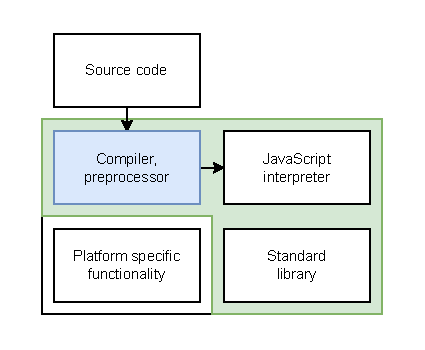
\includegraphics[width=0.7\textwidth, draft=false]{assets/img/overview.pdf}
    \caption{Overview of the changes to Jaculus. In green is highlighted a platform-independent part of the runtime environment -- Jaculus-machine. The preprocessing step represents the changes added to Jaculus-machine in this thesis.}
    \label{fig:overview}
\end{figure}
